
\begin{figure*}[!t]
  \begin{threeparttable}
  \captionof{table}{Data Scheduling Semantics Example Function, $f$: Definition and Implementations}
  \label{tbl:DataSchedDefImpl}
  \setlength\tabcolsep{1.5pt}
  \begin{tabular}{|c|c|c|c|c|}
  \hline 
  \textbf{Formal Definition} & \textbf{Functional Drawing} & \textbf{C++ Impl.}\tnote{†} & \textbf{VHDL Impl.\tnote{‡}} & \textbf{DFiant Impl.} \\ 
  \hline
	\begin{minipage}[b]{0.23\linewidth}
    {\fontsize{8}{8}\selectfont
    \begin{equation}    
      \nonumber
      \begin{aligned}
        &f:(i_{n})_{n\in \mathbb{N}}\rightarrow (a_n,b_n,c_n,d_n)_{n\in \mathbb{N}}\\ 
        &\triangleq\left\{
        \begin{split}
          a_k & = i_k + 5 \\
          b_k & = a_k * 3 \\
          c_k & = a_k + b_k \\
          d_k & = i_k - 1 \\
        \end{split}\right.k\geq 0 \\
        \\
      \end{aligned}
    \end{equation}
    }
	\end{minipage}
  &
	\begin{minipage}[b][3.2cm][c]{0.18\linewidth}
    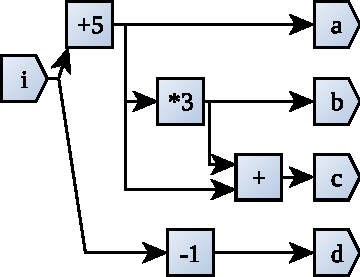
\includegraphics[width=\linewidth]{graphics/fFuncDraw.pdf}
  \end{minipage}%
  &
	\begin{minipage}[b]{0.18\linewidth}
		\begin{minted}[autogobble,tabsize=2,fontsize=\fontsize{8}{8}\selectfont]{c}
      void f(int i,
             &a,&b,&c,&d){ 
      
      
        a = i + 5;
        b = a * 3;
      
        c = a + b;
        d = i - 1;

      }
		\end{minted}
	\end{minipage}
	&
	\begin{minipage}[b]{0.18\linewidth}
		\begin{minted}[autogobble,tabsize=2,fontsize=\fontsize{8}{8}\selectfont]{vhdl}
      f : process(clk)
      begin 
        if rising_edge(clk)
        begin
          a <= i + 5;
          b <= a * 3;
          â <= a;--cyc delay
          c <= â + b;
          d <= i - 1;
        end; 
      end process;
		\end{minted}
	\end{minipage}
	&
	\begin{minipage}[b]{0.19\linewidth}
		\begin{minted}[autogobble,tabsize=2,fontsize=\fontsize{8}{8}\selectfont]{scala}
      def f(i : DFSInt[32]) = 
      {
      
      
        val a = i + 5
        val b = a * 3
      
        val c = a + b
        val d = i - 1
        (a,b,c,d) //tuple of
      }           //four
		\end{minted}
	\end{minipage}
  \\
  \hline
  \end{tabular}
  \begin{tablenotes}
    \item [†] Some type annotations were removed for brevity.
    \item [‡] \textbf{â} represents a clock cycle delay of \textbf{a}.
  \end{tablenotes}
  \end{threeparttable}
\end{figure*}%
